\documentclass[
	a4paper, % Paper size, use either a4paper or letterpaper
	10pt, % Default font size, can also use 11pt or 12pt, although this is not recommended
	unnumberedsections, % Comment to enable section numbering
	twoside, % Two side traditional mode where headers and footers change between odd and even pages, comment this option to make them fixed
]{LTJournalArticle}

\addbibresource{sample.bib} % BibLaTeX bibliography file

% A shortened article title to appear in the running head, leave this command empty for no running head

% \footertext{\textit{Journal of Biological Sampling} (2024) 12:533-684} % Text to appear in the footer, leave this command empty for no footer text

\setcounter{page}{1} % The page number of the first page, set this to a higher number if the article is to be part of an issue or larger work

%----------------------------------------------------------------------------------------
%	TITLE SECTION
%----------------------------------------------------------------------------------------

\title{Probabilistic Approaches to 
\\ Energy Conservation in CDNs} % Article title, use manual lines breaks (\\) to beautify the layout

% Authors are listed in a comma-separated list with superscript numbers indicating affiliations
% \thanks{} is used for any text that should be placed in a footnote on the first page, such as the corresponding author's email, journal acceptance dates, a copyright/license notice, keywords, etc
\author{%
	Adarsh Hiremath, Artemas Radik, Andrew Palacci \\
	CS 262: Introduction to Distributed Systems \\
}


%----------------------------------------------------------------------------------------

\begin{document}

\maketitle % Output the title section

%----------------------------------------------------------------------------------------
%	ARTICLE CONTENTS
%----------------------------------------------------------------------------------------

\begin{abstract}
\end{abstract}
\section{1. Introduction}

\section{2. Existing Methods}
Notes / plans for this section: 
\begin{enumerate}
    \item 
\end{enumerate}

\section{3. The Need for a New Cache Policy}

Caching content strategically is crucial for highly performant CDNs. 

\begin{figure}[h]
	\begin{center}
		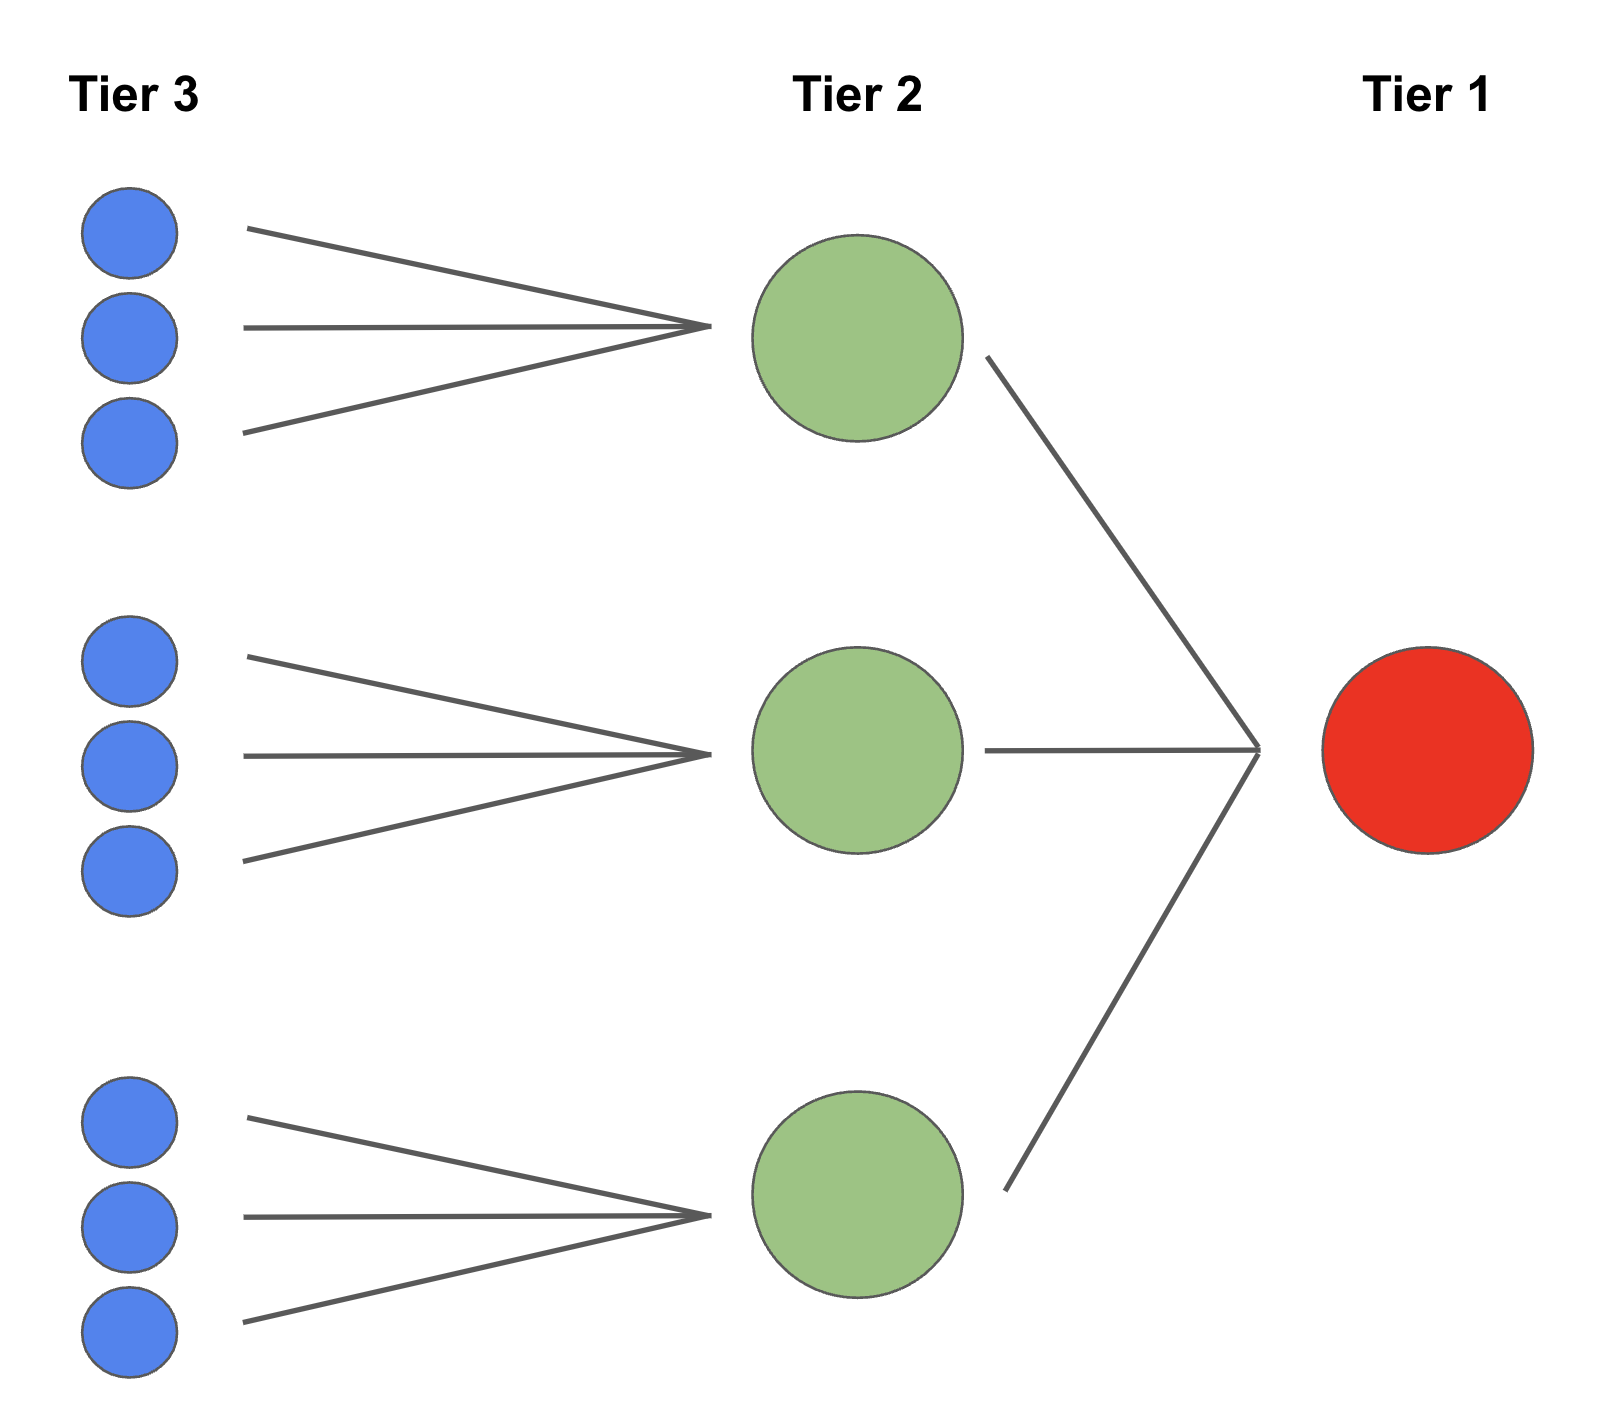
\includegraphics[width=8.1cm]{tier.png}
	\end{center}
	\caption{A diagram of a 3-tier CDN.}
	\label{fig:tier-cdn}	
\end{figure}

% \section{x. Pareto/Bimodal Energy Consumption}

% \section{x. Samples at Scale} (potentially)

% \section{Adaptations to the current model}
% in this section, we can talk about 1. having a crossover point where adding more servers is not energy effective, 2. how we would incorporate this into our model using an additional dependency on S in the server energy 
% include a real world example analogous to the Youtube example in the current paper we are using --- use this ratio of r_m to m_m to calculate where the crossover point would be, and note that a similar strategy could be implemented by CDN users to optimize their energy consumption

% \section{x. Future Work}

% \section{x. References}


\end{document}
